\section{Merge Sort}
L'algoritmo di ordinamento per fusione si basa sul seguente schema:
\begin{itemize}
    \item Un array di un solo elemento è già ordinato (\emph{caso base})
    \item Per ordinare un array $A$ contenente $n > 1$ elementi possiamo:
    \begin{enumerate}
        \item suddividere $A$ in due array $B$ e $C$ di $n/2$ elementi ciascuno,
        corrispondenti alla prima e alla seconda metà dell'array $A$ (Nel caso $n$ 
        sia dispari le due metà saranno di $\lfloor n/2 \rfloor$ e $\lceil n/2 \rceil$ )
        \item ordinare separatamente gli array
        \item "fondere" gli array ordinati $B$ e $C$ nell'array $A$, in modo da
        ottenere un array ordinato contenente gli elementi di $B$ e $C$.
    \end{enumerate}
\end{itemize}

\noindent L'operazione di fusione ({\texttt{merge}}) di due array ordinati
in un array ordinato è più semplice rispetto all'ordinamento di un array.

\noindent Studiamo come effettuare il merge. Disponiamo di due vettori $B$ e $C$ ordinati
in modo non decrescente, e vogliamo ottenere un vettore $X$ ordinato che contenga
gli stessi elementi di $B$ e $C$.

\begin{enumerate}
    \item Creiamo un vettore $X$ la cui lunghezza sia la somma delle lunghezze di 
    $B$ e $C$
    \item Ispezioniamo $B$ e $C$ iniziando a considerare gli elementi minimi, ovvero quelli
    nella prima posizione dei due vettori
    \item Confrontiamo i due elementi e scegliamo il minimo, copiandolo nella 
    prima posizione libera di $X$. Inoltre, nel vettore da cui abbiamo preso
    l'elemento, possiamo considerare quello di posizione successiva.
    \item Ripetiamo le operazioni precedenti fino a raggiungere la fine di uno dei due array
    \item Copiamo in $X$ tutti gli elementi rimanenti dell'altro array
\end{enumerate}

\subsubsection*{Numero di confronti}
Indicando con $C(n)$ il numero di confronti effettuato da {\texttt{mergeSort}}
possiamo scrivere la seguente equazione di ricorrenza.

\begin{equation*}
    C(n)=\begin{cases}
        C(\lfloor n/2 \rfloor) + C(\lceil n/2 \rceil) + C_{\texttt{merge}}(n) & \text{se $n > 1$}\\
        0 & \text{altrimenti}
    \end{cases}
\end{equation*}

Nel caso peggiore $C_{\texttt{merge}}(n) = n - 1$. Risolvendo per sostituzione
otteniamo $C(n) = \Theta(n \log n)$

\subsubsection*{Tempo di calcolo}
Ci sono varie operazioni costose sia in termini di tempo che in termini di spazio:
dobbiamo creare due array $B$ e $C$, copiarvi gli elementi di $A$ e, dopo il 
merge, ricopiare tutti gli elementi nell'array iniziale. Indicando con $T(n)$ il tempo
utilizzato dall'algoritmo per ordinare un array di lunghezza $n$ osserviamo che:
\begin{itemize}
    \item Se l'array contiene al più 1 elemento, l'algoritmo usa tempo costante.
    Indichiamo tale tempo con $a$
    \item Se l'array contiene $n > 1$ elementi, allora $T(n)$ è la somma dei seguenti tempi:
    \begin{itemize}
        \item Tempo per la creazione dei due array: $\Theta(n)$
        \item Tempo per ordinare i due array: $T(\lfloor n/2 \rfloor) + T(\lceil n/2 \rceil)$
        \item Tempo per il merge: $\Theta(n)$
    \end{itemize}

\end{itemize}
\noindent Possiamo quindi scrivere l'equazione di ricorrenza
\begin{equation*}
    T(n)=\begin{cases}
        2T(n/2) + bn + c & \text{se $n > 1$}\\
        a & \text{altrimenti}
    \end{cases}
\end{equation*}
dove $b$ e $c$ sono due costanti.\\
Risolvendo per sostituzione ottengo $T(n) = \Theta(n \log n)$

\subsubsection*{Implementazione}
Come abbiamo visto, l'implementazione di una versione base di {\texttt{mergeSort}}
richiede l'uso di tempo e spazio per gli array $B$ e $C$. Possiamo implementare
l'algoritmo in maniera differente, servendoci direttamente dell'array $A$ da ordinare
e di due indici che delimitano la parte da ordinare.
Al contrario, per effettuare la procedura {\texttt{merge}} ci serviremo di un 
array ausiliario, che per evitare sprechi verrà creato preliminarmente
e verrà usato da tutte le chiamate di {\texttt{merge}}.
La precedente analisi relativa al numero di confronti non cambia e il tempo
rimane dell'ordine di $n \log n$.

\begin{figure}[h]
    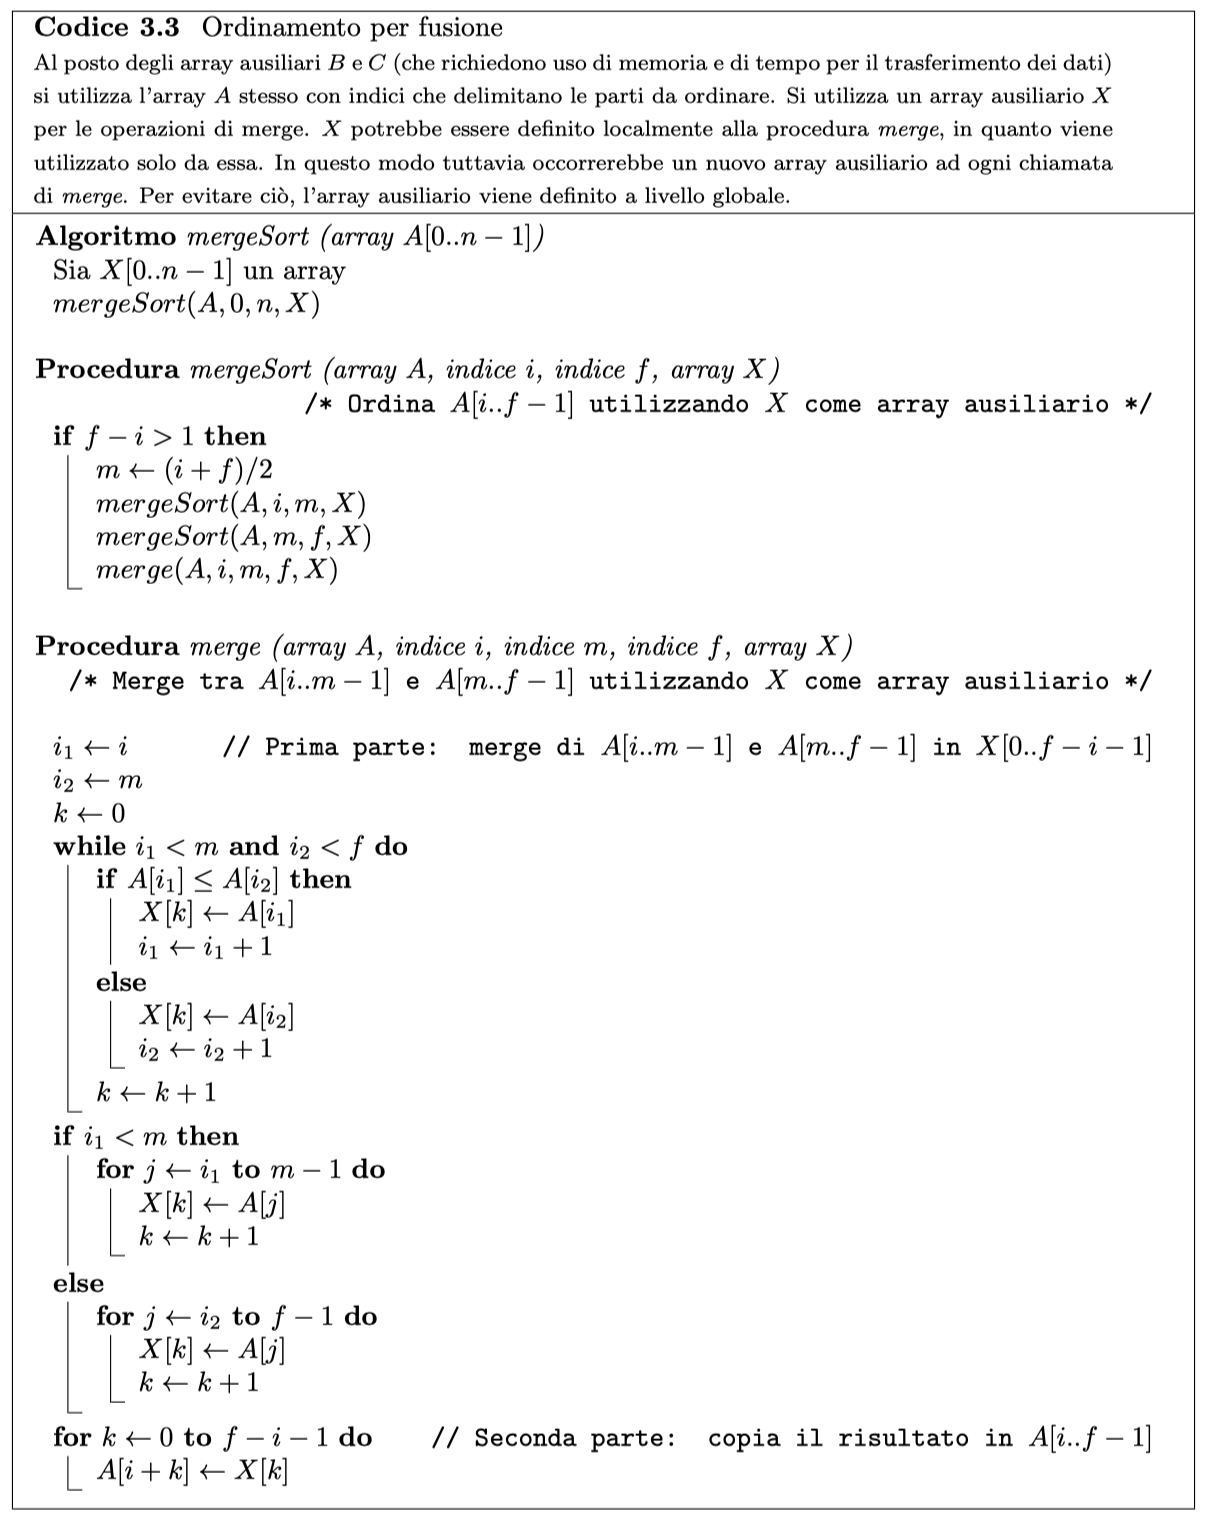
\includegraphics[width=\textwidth]{mergesort.png}
\end{figure}

\clearpage

\subsubsection*{Spazio}
L'algoritmo non è in loco, in quanto utilizza un array ausiliario per effettuare
il merge. L'array è di $n$ elementi, quindi usa spazio $\Theta(n)$.
Dobbiamo inoltre considerare lo spazio utilizzato dallo stack per gestire la ricorsione.
In ciascun record di attivazione di {\texttt{mergeSort}} devono essere memorizzati
gli indici $i$ ed $f$ che servono a delimitare la porzione di array da delimitare e la 
variabile $m$. Pertanto la dimensione di ogni record è costante. Per calcolare l'altezza
dello stack utilizziamo un'equazione di ricorrenza.
\begin{itemize}
    \item Se $n \le 1$ (caso base) non viene effettuata alcuna chiamata ricorsiva.
    Pertanto viene utilizzato solo il record di attivazione corrente e $H(n) = 1$
    \item Se $n > 1$ viene effettuata una prima chiamata ricorsiva su un array di 
    lunghezza $\lfloor n/2 \rfloor$, che dunque utilizzerà altezza $H(\lfloor n/2 \rfloor)$.
    terminata tale chiamata si effettua una seconda chiamata sull'altra parte di array,
    quindi con altezza $H(\lceil n/2 \rceil)$. Poichè al termine di ciascuna
    chiamata ricorsiva lo stack viene riportato all'altezza che aveva prima della chiamata,
    la parte di stack utilizzata dalla prima chiamata viene riutilizzata per la seconda.
    Pertanto l'altezza dello stack utilizzata dalle due chiamate è il massimo tra 
    $H(\lfloor n/2 \rfloor)$ e $H(\lceil n/2 \rceil)$.
\end{itemize}

\noindent Otteniamo dunque 
\begin{equation*}
    H(n) = \begin{cases}
        max(H(\lfloor n/2 \rfloor), H(\lceil n/2 \rceil)) + 1 & \text{se $n > 1$}\\
        1 & \text{altrimenti}
    \end{cases}
\end{equation*}

Questo ci permette di concludere che l'altezza dello stack è logaritmica rispetto a n, 
ed è in particolare $\Theta(\log n)$.
\clearpage
